% !TEX root = ./FT_II-Slides_Annotations.2024.1.7.tex
\providecommand\mainfilename{"./FT_II-Slides_Annotations.tex"}
\providecommand \subfilename{}
\renewcommand   \subfilename{"./FT_II-Slides_Annotations.2024.1.7.tex"}
\documentclass[\mainfilename]{subfiles}

% \tikzset{external/force remake=true} % - remake all

\begin{document}

\graphicspath{{\subfix{./figures/FT_II-Slides_Annotations.2024.1.7}}}
% \tikzsetexternalprefix{./figures/FT_II-Slides_Annotations.2024.1.7/graphics/}

\stepcounter{part}
\mymakesubfile{\arabic{part}}
[FT II]
{Slides 2024: Difusão em Estado Transiente} % Subfile Title
{Slides 2024: Difusão em Estado Transiente} % Part Title

\begin{sectionBox}{Caracteristicas} % MARK: S
    
    \begin{itemize}
        \item Em processos transisentes a concentração num determinado ponto/posição varia com o tempo
        \item Estado não estacionário: Processo que depende do tempo
    \end{itemize}
    
\end{sectionBox}

\begin{sectionBox}1{Balanço de Massa} % MARK: S
    
    \begin{center}
        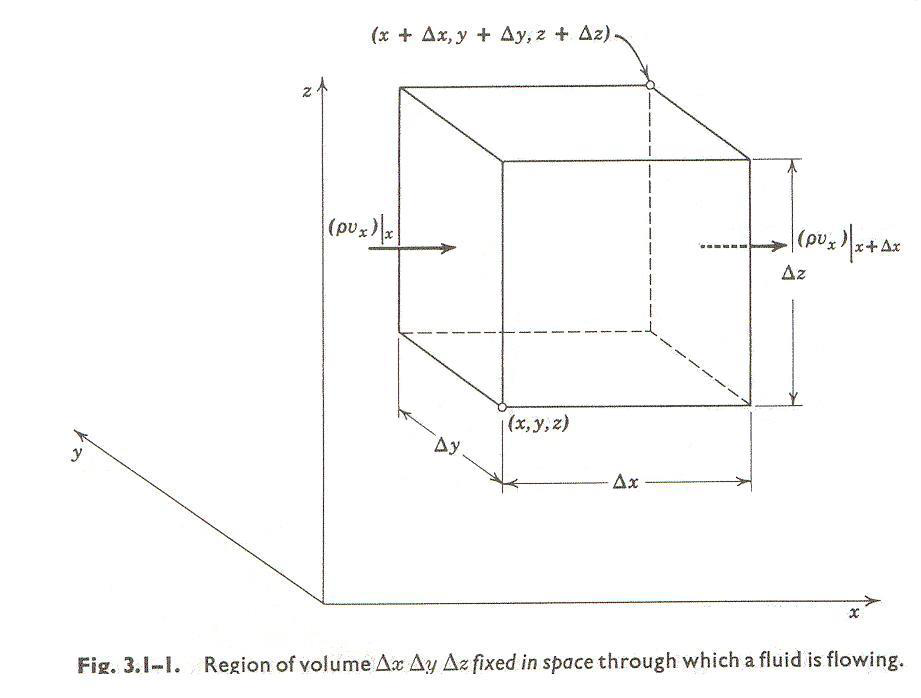
\includegraphics[width=.8\textwidth]{out-003.png}
    \end{center}

    \begin{sectionBox}*2m{Soluções binárias líquidas diluidas} % MARK: S
        \begin{BM}
            \mdv{c_A}{t}
            = \mathscr{D}_{A,B}
            \,\gdif[order=2]{c_A}
            + R_A
        \end{BM}
        \begin{itemize}
            \item \(r_A=-r_B; n_A+n_B=\rho\,v\)
            \item Constantes: \(\rho,\mathscr{D}\)
        \end{itemize}
    \end{sectionBox}

    \begin{sectionBox}*2m{2ª Lei de Fick} % MARK: S
        \begin{BM}
            \pdv{c_A}{t}
            = \mathscr{D}_{A,B}
            \,\gdif[order=2]{c_A}
        \end{BM}
        \begin{itemize}
            \item \(r_A=-r_B; n_A+n_B=\rho\,v\)
            \item Constantes: \(\rho,\mathscr{D}\)
            \item Não reativo \(R_A=R_B=0\)
            \item Sem Movimento \(v=0\)
        \end{itemize}
    \end{sectionBox}

    \paragraph*{Demonstração:}
    
    \begin{BM}
        \text{Acumulação}_A
        = \text{Entrada}_A
        - \text{Saída}_A
        + \text{Prod}_A
    \end{BM}

    \begin{itemize}
        \item Variação de massa de A no elemento de volume:
        \begin{BM}
            \pdv{\rho_A}{t}\,\adif{x,y,z}
        \end{BM}
        \item Entrada de A através da face \textit{x}:
        \begin{BM}
            n_{A,x}\Big\vert_x
            \,\adif{y,z}
        \end{BM}
        \item Saída de massa de A através da face \(x+\adif{x}\):
        \begin{BM}
            n_{A,x}\Big\vert_{x+\adif{x}}
            \,\adif{y,z}
        \end{BM}
        \item Produção de A por reação química
        \begin{BM}
            r_A\,\adif{x,y,z}
        \end{BM}
        \item \(\dim{r_A}=\unit{\gram/\metre^3.\hour}\): Massa de A produzido por volume e tempo
        \item \(n_{A,i}\): Componentes do vetor fluxo de massa
    \end{itemize}

    \begin{flalign*}
        &
            \pdv{\rho_A}{t}
            \,\adif{x,y,z}
            = \left(
                \begin{aligned}
                    &
                        \adif{y,z}\left(
                            n_{A,x}\Big\vert_x
                            - n_{A,x}\Big\vert_{x+\adif{x}}
                        \right)
                    &+\\+&
                        \adif{x,z}\left(
                            n_{A,y}\Big\vert_y
                            - n_{A,y}\Big\vert_{y+\adif{y}}
                        \right)
                    &+\\+&
                        \adif{x,y}\left(
                            n_{A,z}\Big\vert_z
                            - n_{A,z}\Big\vert_{z+\adif{z}}
                        \right)
                    &
                \end{aligned}
            \right)
            \implies &\\[3ex]&
            \implies
            r_A
            = \pdv{\rho_A}{t}
            + \left(
                \pdv{n_{A,x}}{x}
                + \pdv{n_{A,y}}{y}
                + \pdv{n_{A,z}}{z}
            \right)
            = \pdv{\rho_A}{t}
            + \gdif{n_A}
        &
    \end{flalign*}

    \subsection*{Adicionando um segundo componente (B)}

    \begin{BM}
        \pdv{\rho}{t}
        + \gdif{(\rho\,v)}
        = 0
    \end{BM}

    \begin{itemize}
        \item Mistura binária: \(n_{A}+n_B=\rho\,v\)
        \item Conservação de massa: \(r_A=-r_B\)
    \end{itemize}

    \paragraph*{Em unidades molares:}
    \begin{BM}
        R_A
        = \pdv{c_A}{t}
        + \gdif{N_A}
        \quad\text{Equação de conservação de A}
        \\
        R_B
        = \pdv{c_B}{t}
        + \gdif{N_B}
        \quad\text{Equação de conservação de B}
        \\
        R_A+R_B
        = \pdv{c}{t}
        + \gdif{c\,v^*}
        \quad\text{Total}
    \end{BM}

    \subsection*{Para obter o perfil de concentrações}

    \paragraph*{Em unidades mássicas:}
    \begin{BM}[align*]
        n_A
        = \omega_A\,(n_A+n_B)
        & - \rho\,\mathscr{D}_{A,B}\,\gdif{\omega_A}
        = \\
        = \rho_A\,v
        & - \rho\,\mathscr{D}_{A,B}\,\gdif{\omega_A}
    \end{BM}

    \paragraph*{Em unidades molares:}
    \begin{BM}
        N_A
        = x_A\,(N_A+N_B)
        - c\,\mathscr{D}_{A,B}\,\gdif{x_A}
    \end{BM}
    
    \subsection*{Substituindo}
    
    \begin{BM}
        \gdif{\rho}
        \,\mathscr{D}_{A,B}
        \,\gdif{\omega_A}
        + r_A
        = \pdv{\rho_A}{t}
        + \gdif{\rho_A\,v}
        \\[3ex]
        \gdif{c_A}
        \,\mathscr{D}_{A,B}
        \,\gdif{x_A}
        + R_A
        = \pdv{c_A}{t}
        + \gdif{c_A\,v^*}
    \end{BM}

    \subsection*{Mantendo \(\rho\) e \(\mathscr{D}\) constantes}
    \begin{BM}
        \mdv{c_A}{t}
        = \mathscr{D}_{A,B}
        \,\gdif[order=2]{c_A}
        + R_A
    \end{BM}

    \begin{flalign*}
        &
            \pdv{\rho}{t}
            + \rho_A\,\gdif{v}
            + v\,\gdif{\rho_A}
            = \mathscr{D}_{A,B}
            \,\gdif[order=2]{\rho_A}
            + r_A
            ; &\\&
            \pdv{\rho}{t}
            + \gdif{\rho\,v}
            = 0
            \implies
            \gdif{v}=0
            \implies &\\[3ex]&
            \implies
            \pdv{c_A}{t}
            + v\,\gdif{c_A}
            = \mathscr{D}_{A,B}
            \,\gdif[order=2]{c_A}
            + R_A
            \implies &\\&
            \implies
            \mdv{c_A}{t}
            = \mathscr{D}_{A,B}
            \,\gdif[order=2]{c_A}
            + R_A
        &
    \end{flalign*}

    \subsection*{Sistema não reativo e sem movimento}

    \paragraph*{2ª lei de Fick}
    \begin{BM}
        \pdv{c_A}{t}
        = \mathscr{D}_{A,B}
        \,\gdif[order=2]{c_A}
    \end{BM}

    \begin{itemize}
        \item Não reativo: \(R_A=R_B=0\)
        \item Sem movimento: \(v=0\)
    \end{itemize}

\end{sectionBox}

\begin{sectionBox}2{Difusão num meio semi--infinito} % MARK: S
    
    \paragraph*{Condições} da 2ª lei de Fick
    \paragraph*{Estados:}
    \begin{center}
        \vspace{1ex}
        \begin{tabular}{l C C C}
            \toprule
            
                \multicolumn{1}{c}{Condição}
                & t
                & z
                & c_A
            
            \\\midrule
            
                Inicial 
                & t=0
                & 0\leq z\leq L
                & c_{A,0}
                \\ Fronteira 1
                & t>0
                & z=0
                & c_{A,s}
                \\ Fronteira 2
                & t>0
                & z\to\infty
                & c_{A,0}
            
            \\\bottomrule
        \end{tabular}
        \vspace{2ex}
    \end{center}

    \begin{center}
        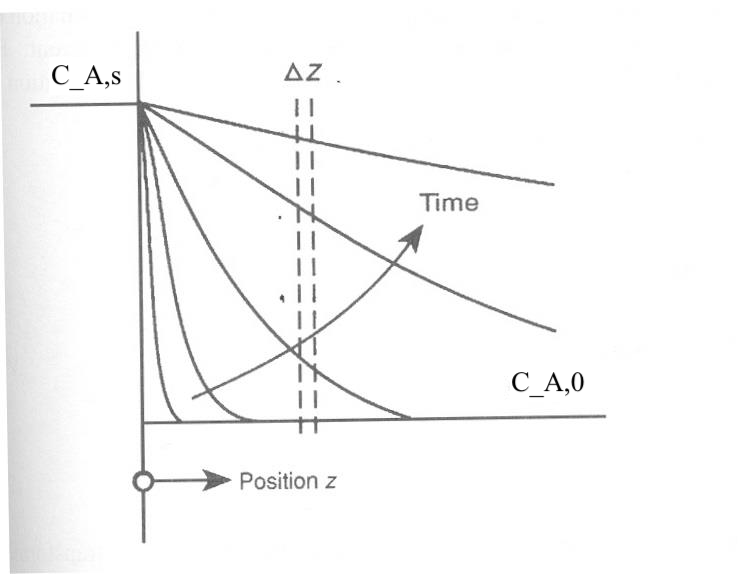
\includegraphics[width=.6\textwidth]{out-012.png}
    \end{center}

    \paragraph*{Solução}
    \begin{BM}
        \odv[order=2]{c_A}{\xi}
        + 2\,\xi
        \,\odv{c_A}{\xi}
        \qquad
        \xi=\frac{z}{\sqrt{4\,\mathscr{D}\,t}}
        \\
        \erf{\xi}
        = \frac{c_{A,s}-c_A}{c_{A,s}-c_{A,0}}
        = \frac{2}{\sqrt{\pi}}
        \,\int_0^{\xi}{
            \exp{-s^2}\,\odif{s}
        }
        \\
        \erf{\myvert{a}}
        = 1-\left(
            \begin{aligned}
                &
                    1
                &+\\+&
                    0.2784\,\myvert{a}
                &+\\+&
                    0.2314\,\myvert{a}^2
                &+\\+&
                    0.0781\,\myvert{a}^4
                &
            \end{aligned}
        \right)^{-4}
    \end{BM}

    \paragraph*{erf:} função erro, valor pode ser usado a tabela para conferir

    \begin{flalign*}
        &
            \odv{c_A}{t}
            = \odv{c_A}{\xi}
            \,\odv{\xi}{t}
            % = &\\&
            = \mathscr{D}_{A,B}
            \,\odv[order=2]{c_A}{z}
            = \mathscr{D}_{A,B}
            \,\odv[order=2]{c_A}{\xi}
            \,\odv[order=2]{\xi}{z}
            ; 
            \qquad
            \xi=\frac{z}{\sqrt{4\,\mathscr{D}\,t}}
            \implies &\\[2ex]&
            \implies
            \odv[order=2]{c_A}{\xi}
            + 2\,\xi
            \,\odv{c_A}{\xi}
        &
    \end{flalign*}

    \subsection*{Fluxo de A:}
    \begin{BM}
        J_A^* 
        = -\mathscr{D}
        \,\pdv{c_A}{z}
        = \sqrt{\frac{\mathscr{D}}{\pi\,t}}
        \,\exp{\left(
            \frac{-z^2}{4\,\mathscr{D}\,t}
        \right)}
        \,(c_{A,s}-c_{A,0})
        \\
        J_A^*\Big\vert_{z=0}
        = \sqrt{\frac{\mathscr{D}}{\pi\,t}}
        \,(c_{A,s}-c_{A,0})
    \end{BM}
    
\end{sectionBox}

\end{document}